\section{Introduction}
\label{sec:introduction}

\begin{figure*}[t]
\centering
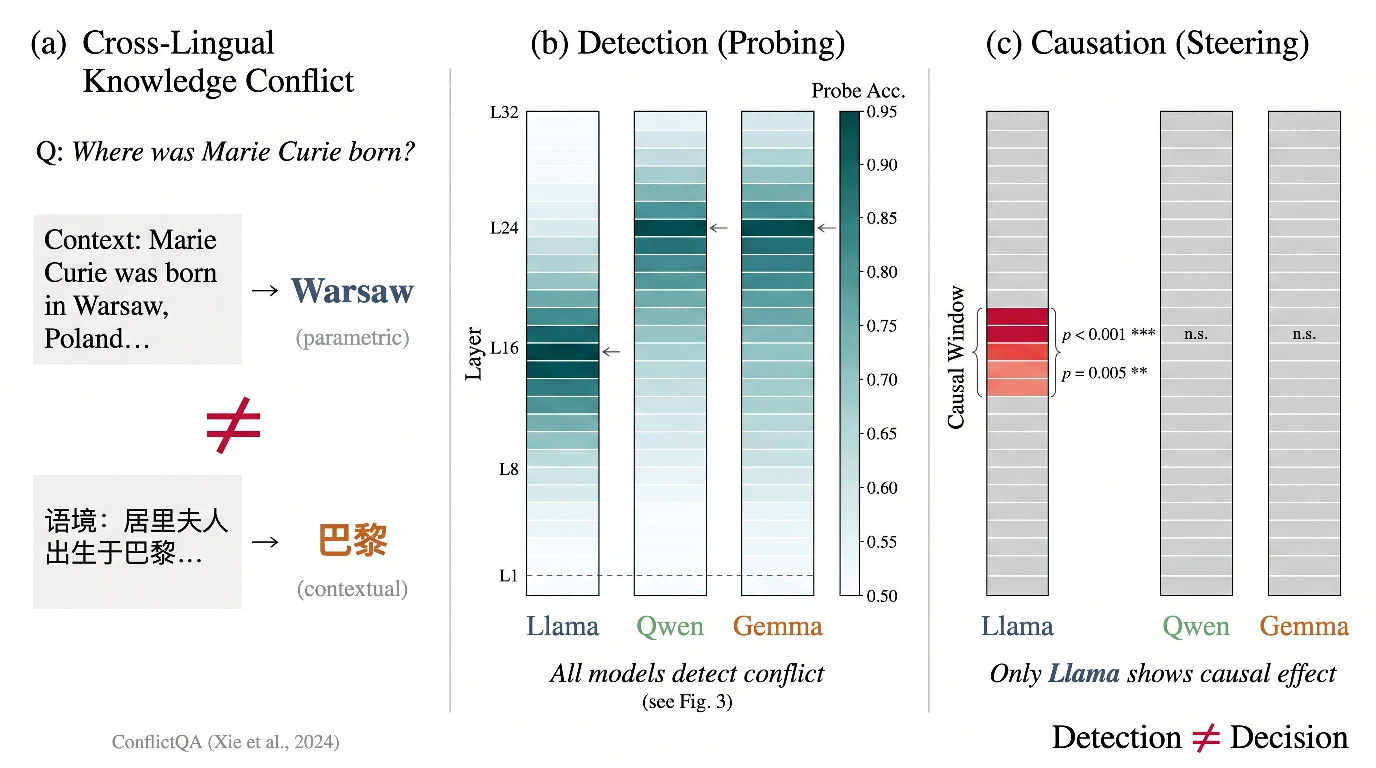
\includegraphics[width=\textwidth]{fig1_hero.pdf}
\caption{Cross-lingual knowledge conflict in multilingual LLMs. When a context passage contradicts the model's parametric knowledge, the language of presentation (English vs.\ Chinese) can bias the answer toward different sources. We ask three questions: (1)~Is the conflict signal linearly detectable in the residual stream? (2)~Do probes transfer across languages, and is the transfer symmetric? (3)~Does detection imply causal influence on resolution?}
\label{fig:hero}
\end{figure*}

When multilingual large language models (LLMs) encounter conflicting information between languages, the language of presentation can determine which answer the model produces \citep{zhao2026when}.
Yet the internal mechanism remains opaque: how does the model encode the conflict signal, can it be detected from internal representations, and does the detected signal causally influence resolution?

Existing work on probing conflict signals has been limited to monolingual settings \citep{zhao2024analysing, brink2026probing}.
Extending cross-lingually introduces confounds (translation quality, token overlap, general transfer properties), and probing establishes correlation rather than causation \citep{hewitt2019designing}; \citet{basu2026interpretability} showed that near-perfect probe accuracy does not guarantee effective steering.

Our work extends \citet{zhao2024analysing} in four directions: (1)~cross-lingual expansion from monolingual English to EN-ZH conflict probing; (2)~a systematic confound exclusion pipeline; (3)~the XNLI baseline revealing that asymmetry parallels general cross-lingual structure; and (4)~three-model causal intervention demonstrating that detectability does not predict causal relevance.
We combine residual stream probing with representation steering across Llama-3.1-8B-Instruct, Qwen3-8B, and Gemma-2-9B-IT.
Probes achieve 77.6\%, 75.0\%, and 76.2\% balanced accuracy on English conflict detection, and all cross-lingual transfer directions exceed chance (binomial $p < 0.001$).
Cross-lingual transfer exhibits a directional asymmetry (ZH$\to$EN $>$ EN$\to$ZH by ${\sim}$7 percentage points [pp]) that is consistent with the XNLI non-conflict baseline \citep{conneau2018xnli}, reflecting general cross-lingual structure rather than conflict-specific encoding.
Our causal analysis reveals a dissociation in Llama: the probe signal peaks at L15 (47\% depth), but steering succeeds only at L13 (41\% depth; Fisher $p < 0.001$), and upper-layer interventions produce no significant change (Figure~\ref{fig:hero}).

Our contributions are as follows:
\begin{itemize}
    \item \textbf{Cross-lingual conflict detectability.} First evidence that knowledge conflict signals are linearly detectable across English and Chinese, with all transfer directions exceeding chance (binomial $p < 0.001$).
    \item \textbf{Asymmetry reflects general cross-lingual structure.} The transfer asymmetry (ZH$\to$EN $>$ EN$\to$ZH by ${\sim}$7~pp) matches the XNLI non-conflict baseline, consistent with general cross-lingual alignment rather than conflict-specific encoding.
    \item \textbf{Detection--decision dissociation.} Linear probe peak (L15), MLP probe peak (L18), and causal steering node (L13; Fisher $p < 0.001$) occupy distinct mid-layers in Llama; the strongest evidence comes from cross-model contrast---all three models detect conflict signals, yet only Llama shows causal steering effects. Steering fails in Gemma despite 88.9\% probe accuracy, providing mechanistic layer-level localization beyond prior behavioral observations \citep{basu2026interpretability}.
    \item \textbf{Confound exclusion pipeline.} COMET translation quality ablation, token overlap analysis, and non-conflict baseline comparison exclude common confounds in cross-lingual probing.
\end{itemize}
